\documentclass[tikz,border=5pt]{standalone}
\usepackage[UTF8]{ctex}
\usepackage{amsmath}
\usetikzlibrary{arrows.meta,calc}
\definecolor{ink}{HTML}{243447}
\definecolor{blue}{HTML}{2765A2}
\definecolor{green}{HTML}{3F7D5B}
\definecolor{red}{HTML}{B74739}
\tikzset{body/.style={draw=ink,thick},vec/.style={blue,thick,-{Latex}},guide/.style={gray!65,dashed},line cap=round}
\newcommand{\cylinder}[2]{
\draw[guide,domain=205.35:385.35,samples=60]plot({.95*cos(\x)+.45*sin(\x)},{.18*cos(\x)-.32*sin(\x)+.60*#1});
\draw[body,domain=25.35:205.35,samples=60]plot({.95*cos(\x)+.45*sin(\x)},{.18*cos(\x)-.32*sin(\x)+.60*#1});
\draw[body,domain=0:360,samples=90]plot({.95*cos(\x)+.45*sin(\x)},{.18*cos(\x)-.32*sin(\x)+.60*#2});
\draw[body](-1.051,-.025+.60*#1)--(-1.051,-.025+.60*#2);
\draw[body](1.051,.025+.60*#1)--(1.051,.025+.60*#2);
}
\begin{document}
\begin{tikzpicture}[scale=1.5]
\cylinder{-1.7}{2.6}
\draw[guide](0,-1.45)--(0,2.1);
\draw[vec](0,1.6)--(0,2.35)node[above]{$z$};
\draw[vec](0,0)--(1.9,.36)node[right]{$x$};
\draw[vec](0,0)--(.9,-.64)node[below]{$y$};
\draw[red,very thick,-{Latex}](-2.5,1)--(-1.4,1.208)node[midway,above]{$\boldsymbol B=B\boldsymbol e_x$};
\fill[blue](.95,.18)circle(1.5pt);
\node[blue,above left]at(.7,.45){$\phi(0)=0$};
\draw[guide](.7,.4)--(.95,.18);
\draw[green,thick,-{Latex}](.95,.18)--(1.7,-.353)node[right]{$R_0\omega_\phi\boldsymbol e_\phi$};
\draw[green,thick,-{Latex}](.95,.18)--(.95,.92)node[left]{$R_0\omega_z\boldsymbol e_z$};
\draw[ink,<->](0,-1.3)--(.95,-1.12)node[midway,below]{$R_0$};
\node at(0,-2.1){光滑圆柱面，径向约束维持半径};
\end{tikzpicture}
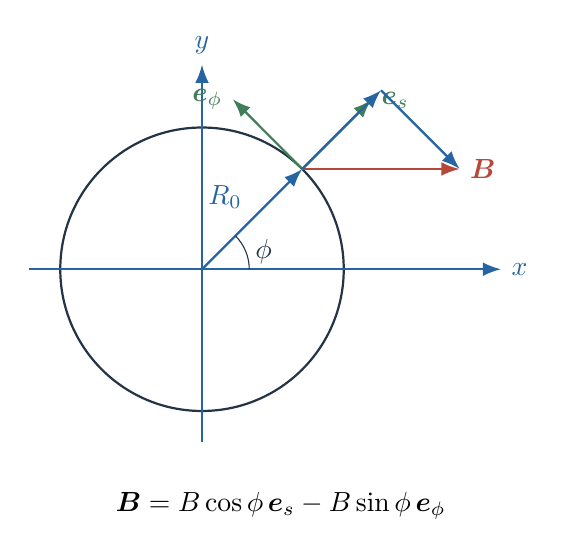
\begin{tikzpicture}
\draw[body](0,0)circle(1.8);
\draw[vec](-2.2,0)--(3.8,0)node[right]{$x$};
\draw[vec](0,-2.2)--(0,2.6)node[above]{$y$};
\coordinate(A)at(1.273,1.273);
\draw[vec](0,0)--(A)node[midway,above left]{$R_0$};
\draw[green,thick,-{Latex}](A)--(2.15,2.15)node[right]{$\boldsymbol e_s$};
\draw[green,thick,-{Latex}](A)--(.39,2.16)node[left]{$\boldsymbol e_\phi$};
\draw[red,thick,-{Latex}](A)--(3.273,1.273)node[right]{$\boldsymbol B$};
\draw[guide](2.273,2.273)--(3.273,1.273);
\draw[blue,thick,-{Latex}](A)--(2.273,2.273);
\draw[blue,thick,-{Latex}](2.273,2.273)--(3.273,1.273);
\draw[ink](.6,0)arc(0:45:.6)node[midway,right]{$\phi$};
\node at(1,-3){$\boldsymbol B=B\cos\phi\,\boldsymbol e_s-B\sin\phi\,\boldsymbol e_\phi$};
\end{tikzpicture}
\begin{tikzpicture}
\begin{scope}[scale=1.05]
\cylinder{-.8}{8.2}
\draw[blue,very thick,densely dashed] plot coordinates {(0.95000000,0.18000000) (0.96165943,0.18091697) (0.97268530,0.18154283) (0.98305925,0.18188233) (0.99276333,0.18194065) (1.00178004,0.18172338) (1.01009240,0.18123654) (1.01768396,0.18048655) (1.02453887,0.17948026) (1.03064192,0.17822491) (1.03597860,0.17672817) (1.04053510,0.17499808) (1.04429840,0.17304309) (1.04725627,0.17087201) (1.04939734,0.16849403) (1.05071110,0.16591871) (1.05118798,0.16315593)};
\draw[blue,very thick] plot coordinates {(1.05118798,0.16315593) (1.05081934,0.16021593) (1.04959751,0.15710924) (1.04751583,0.15384671) (1.04456866,0.15043949) (1.04075140,0.14689899) (1.03606054,0.14323686) (1.03049361,0.13946502) (1.02404927,0.13559559) (1.01672727,0.13164088) (1.00852845,0.12761341) (0.99945481,0.12352585) (0.98950943,0.11939101) (0.97869652,0.11522182) (0.96702143,0.11103132) (0.95449058,0.10683265) (0.94111153,0.10263900) (0.92689290,0.09846359) (0.91184442,0.09431970) (0.89597688,0.09022058) (0.87930211,0.08617950) (0.86183298,0.08220968) (0.84358337,0.07832428) (0.82456818,0.07453642) (0.80480323,0.07085910) (0.78430534,0.06730523) (0.76309222,0.06388761) (0.74118248,0.06061888) (0.71859560,0.05751153) (0.69535190,0.05457787) (0.67147251,0.05183005) (0.64697934,0.04927997) (0.62189505,0.04693936) (0.59624302,0.04481967) (0.57004730,0.04293212) (0.54333262,0.04128769) (0.51612430,0.03989705) (0.48844826,0.03877059) (0.46033098,0.03791841) (0.43179943,0.03735028) (0.40288107,0.03707565) (0.37360381,0.03710362) (0.34399597,0.03744296) (0.31408622,0.03810206) (0.28390358,0.03908894) (0.25347735,0.04041126) (0.22283709,0.04207627) (0.19201258,0.04409080) (0.16103376,0.04646131) (0.12993070,0.04919381) (0.09873360,0.05229391) (0.06747266,0.05576676) (0.03617812,0.05961710) (0.00488018,0.06384918) (-0.02639104,0.06846685) (-0.05760555,0.07347348) (-0.08873352,0.07887197) (-0.11974532,0.08466477) (-0.15061158,0.09085387) (-0.18130324,0.09744077) (-0.21179157,0.10442653) (-0.24204822,0.11181174) (-0.27204530,0.11959649) (-0.30175536,0.12778044) (-0.33115149,0.13636277) (-0.36020735,0.14534222) (-0.38889717,0.15471706) (-0.41719585,0.16448513) (-0.44507897,0.17464380) (-0.47252281,0.18519005) (-0.49950442,0.19612040) (-0.52600167,0.20743098) (-0.55199320,0.21911751) (-0.57745855,0.23117531) (-0.60237814,0.24359935) (-0.62673329,0.25638420) (-0.65050627,0.26952411) (-0.67368030,0.28301299) (-0.69623958,0.29684443) (-0.71816933,0.31101170) (-0.73945575,0.32550781) (-0.76008607,0.34032549) (-0.78004857,0.35545724) (-0.79933253,0.37089531) (-0.81792831,0.38663175) (-0.83582727,0.40265842) (-0.85302182,0.41896699) (-0.86950540,0.43554900) (-0.88527247,0.45239586) (-0.90031847,0.46949884) (-0.91463988,0.48684913) (-0.92823410,0.50443786) (-0.94109953,0.52225607) (-0.95323546,0.54029480) (-0.96464212,0.55854504) (-0.97532061,0.57699779) (-0.98527287,0.59564406) (-0.99450168,0.61447489) (-1.00301059,0.63348136) (-1.01080392,0.65265464) (-1.01788671,0.67198593) (-1.02426469,0.69146655) (-1.02994422,0.71108791) (-1.03493229,0.73084154) (-1.03923645,0.75071907) (-1.04286479,0.77071229) (-1.04582592,0.79081312) (-1.04812886,0.81101364) (-1.04978309,0.83130606) (-1.05079845,0.85168279) (-1.05118515,0.87213640)};
\draw[blue,very thick,densely dashed] plot coordinates {(-1.05118515,0.87213640) (-1.05095367,0.89265961) (-1.05011478,0.91324536) (-1.04867949,0.93388674) (-1.04665900,0.95457704) (-1.04406467,0.97530973) (-1.04090802,0.99607848) (-1.03720063,1.01687712) (-1.03295417,1.03769971) (-1.02818038,1.05854045) (-1.02289096,1.07939376) (-1.01709763,1.10025423) (-1.01081208,1.12111663) (-1.00404591,1.14197592) (-0.99681066,1.16282720) (-0.98911776,1.18366578) (-0.98097850,1.20448712) (-0.97240405,1.22528682) (-0.96340541,1.24606068) (-0.95399341,1.26680462) (-0.94417870,1.28751470) (-0.93397171,1.30818714) (-0.92338269,1.32881829) (-0.91242165,1.34940462) (-0.90109837,1.36994272) (-0.88942241,1.39042931) (-0.87740307,1.41086120) (-0.86504942,1.43123531) (-0.85237028,1.45154867) (-0.83937420,1.47179839) (-0.82606950,1.49198165) (-0.81246423,1.51209572) (-0.79856620,1.53213794) (-0.78438294,1.55210572) (-0.76992176,1.57199651) (-0.75518970,1.59180783) (-0.74019358,1.61153723) (-0.72493996,1.63118231) (-0.70943516,1.65074070) (-0.69368531,1.67021006) (-0.67769627,1.68958807) (-0.66147371,1.70887241) (-0.64502311,1.72806080) (-0.62834971,1.74715094) (-0.61145859,1.76614055) (-0.59435463,1.78502733) (-0.57704257,1.80380897) (-0.55952696,1.82248315) (-0.54181221,1.84104754) (-0.52390258,1.85949976) (-0.50580222,1.87783744) (-0.48751516,1.89605813) (-0.46904531,1.91415939) (-0.45039650,1.93213871) (-0.43157249,1.94999356) (-0.41257696,1.96772133) (-0.39341354,1.98531939) (-0.37408582,2.00278505) (-0.35459738,2.02011557) (-0.33495177,2.03730812) (-0.31515254,2.05435986) (-0.29520329,2.07126785) (-0.27510761,2.08802911) (-0.25486917,2.10464057) (-0.23449169,2.12109912) (-0.21397897,2.13740156) (-0.19333490,2.15354464) (-0.17256348,2.16952503) (-0.15166885,2.18533935) (-0.13065526,2.20098411) (-0.10952714,2.21645581) (-0.08828909,2.23175083) (-0.06694590,2.24686552) (-0.04550254,2.26179614) (-0.02396423,2.27653892) (-0.00233641,2.29109000) (0.01937523,2.30544548) (0.04116472,2.31960139) (0.06302584,2.33355373) (0.08495203,2.34729844) (0.10693645,2.36083141) (0.12897193,2.37414852) (0.15105095,2.38724559) (0.17316566,2.40011842) (0.19530782,2.41276280) (0.21746882,2.42517450) (0.23963967,2.43734927) (0.26181098,2.44928288) (0.28397293,2.46097110) (0.30611530,2.47240971) (0.32822744,2.48359453) (0.35029826,2.49452141) (0.37231623,2.50518623) (0.39426939,2.51558494) (0.41614529,2.52571356) (0.43793108,2.53556817) (0.45961342,2.54514496) (0.48117853,2.55444019) (0.50261218,2.56345025) (0.52389969,2.57217167) (0.54502594,2.58060110) (0.56597538,2.58873533) (0.58673203,2.59657133) (0.60727950,2.60410625) (0.62760099,2.61133742) (0.64767932,2.61826239) (0.66749694,2.62487891) (0.68703594,2.63118497) (0.70627811,2.63717882) (0.72520488,2.64285895) (0.74379745,2.64822414) (0.76203674,2.65327344) (0.77990343,2.65800622) (0.79737804,2.66242215) (0.81444089,2.66652122) (0.83107220,2.67030378) (0.84725209,2.67377050) (0.86296062,2.67692242) (0.87817784,2.67976095) (0.89288383,2.68228789) (0.90705874,2.68450541) (0.92068285,2.68641607) (0.93373656,2.68802285) (0.94620051,2.68932912) (0.95805557,2.69033866) (0.96928294,2.69105569) (0.97986412,2.69148483) (0.98978104,2.69163110) (0.99901604,2.69149999) (1.00755199,2.69109735) (1.01537225,2.69042951) (1.02246079,2.68950315) (1.02880219,2.68832542) (1.03438171,2.68690384) (1.03918531,2.68524634) (1.04319973,2.68336123) (1.04641248,2.68125721) (1.04881192,2.67894337) (1.05038726,2.67642914) (1.05112864,2.67372430)};
\draw[blue,very thick] plot coordinates {(1.05112864,2.67372430) (1.05102710,2.67083898) (1.05007469,2.66778361) (1.04826442,2.66456897) (1.04559032,2.66120610) (1.04204747,2.65770631) (1.03763200,2.65408121) (1.03234113,2.65034262) (1.02617315,2.64650260) (1.01912746,2.64257340) (1.01120457,2.63856748) (1.00240611,2.63449747) (0.99273482,2.63037612) (0.98219456,2.62621634) (0.97079031,2.62203115) (0.95852816,2.61783363) (0.94541531,2.61363697) (0.93146005,2.60945439) (0.91667176,2.60529914) (0.90106090,2.60118450) (0.88463897,2.59712371) (0.86741851,2.59313003) (0.84941311,2.58921663) (0.83063731,2.58539665) (0.81110668,2.58168312) (0.79083771,2.57808900) (0.76984784,2.57462710) (0.74815539,2.57131013) (0.72577957,2.56815063) (0.70274045,2.56516097) (0.67905890,2.56235333) (0.65475658,2.55973971) (0.62985594,2.55733189) (0.60438011,2.55514142) (0.57835296,2.55317958) (0.55179898,2.55145743) (0.52474333,2.54998574) (0.49721174,2.54877500) (0.46923051,2.54783538) (0.44082646,2.54717677) (0.41202691,2.54680872) (0.38285963,2.54674045) (0.35335281,2.54698082) (0.32353501,2.54753835) (0.29343515,2.54842118) (0.26308244,2.54963708) (0.23250637,2.55119342) (0.20173665,2.55309718) (0.17080318,2.55535493) (0.13973599,2.55797283) (0.10856525,2.56095660) (0.07732115,2.56431155) (0.04603393,2.56804254) (0.01473381,2.57215398) (-0.01654907,2.57664986) (-0.04778467,2.58153367) (-0.07894309,2.58680849) (-0.10999465,2.59247689) (-0.14090989,2.59854102) (-0.17165964,2.60500253) (-0.20221507,2.61186261) (-0.23254771,2.61912200) (-0.26262950,2.62678096) (-0.29243287,2.63483928) (-0.32193072,2.64329628) (-0.35109653,2.65215085) (-0.37990435,2.66140141) (-0.40832886,2.67104592) (-0.43634542,2.68108190) (-0.46393009,2.69150647) (-0.49105968,2.70231627) (-0.51771178,2.71350757) (-0.54386480,2.72507620) (-0.56949799,2.73701762) (-0.59459149,2.74932691) (-0.61912633,2.76199875) (-0.64308448,2.77502751) (-0.66644885,2.78840718) (-0.68920335,2.80213146) (-0.71133286,2.81619372) (-0.73282328,2.83058706) (-0.75366150,2.84530429) (-0.77383549,2.86033797) (-0.79333420,2.87568043) (-0.81214765,2.89132379) (-0.83026689,2.90725996) (-0.84768400,2.92348067) (-0.86439210,2.93997751) (-0.88038532,2.95674190) (-0.89565880,2.97376518) (-0.91020870,2.99103855) (-0.92403211,3.00855317) (-0.93712714,3.02630009) (-0.94949279,3.04427035) (-0.96112901,3.06245496) (-0.97203661,3.08084491) (-0.98221729,3.09943121) (-0.99167355,3.11820489) (-1.00040871,3.13715702) (-1.00842685,3.15627873) (-1.01573280,3.17556120) (-1.02233205,3.19499574) (-1.02823078,3.21457370) (-1.03343578,3.23428659) (-1.03795444,3.25412599) (-1.04179469,3.27408367) (-1.04496495,3.29415147) (-1.04747414,3.31432145) (-1.04933159,3.33458576) (-1.05054704,3.35493675) (-1.05113057,3.37536694)};
\draw[blue,very thick,densely dashed] plot coordinates {(-1.05113057,3.37536694) (-1.05109259,3.39586901) (-1.05044378,3.41643582) (-1.04919509,3.43706042) (-1.04735765,3.45773603) (-1.04494278,3.47845606) (-1.04196194,3.49921413) (-1.03842671,3.52000401) (-1.03434873,3.54081969) (-1.02973972,3.56165533) (-1.02461139,3.58250527) (-1.01897548,3.60336406) (-1.01284366,3.62422641) (-1.00622758,3.64508721) (-0.99913880,3.66594153) (-0.99158878,3.68678460) (-0.98358885,3.70761185) (-0.97515024,3.72841883) (-0.96628399,3.74920128) (-0.95700100,3.76995506) (-0.94731195,3.79067622) (-0.93722737,3.81136092) (-0.92675756,3.83200545) (-0.91591259,3.85260627) (-0.90470233,3.87315991) (-0.89313640,3.89366307) (-0.88122420,3.91411252) (-0.86897486,3.93450515) (-0.85639727,3.95483796) (-0.84350008,3.97510802) (-0.83029168,3.99531250) (-0.81678020,4.01544865) (-0.80297352,4.03551378) (-0.78887928,4.05550527) (-0.77450483,4.07542058) (-0.75985733,4.09525719) (-0.74494363,4.11501264) (-0.72977040,4.13468453) (-0.71434403,4.15427048) (-0.69867069,4.17376812) (-0.68275634,4.19317514) (-0.66660672,4.21248923) (-0.65022734,4.23170808) (-0.63362354,4.25082940) (-0.61680044,4.26985091) (-0.59976299,4.28877032) (-0.58251596,4.30758531) (-0.56506396,4.32629358) (-0.54741144,4.34489280) (-0.52956272,4.36338059) (-0.51152198,4.38175460) (-0.49329328,4.40001239) (-0.47488057,4.41815153) (-0.45628770,4.43616952) (-0.43751846,4.45406383) (-0.41857654,4.47183190) (-0.39946560,4.48947109) (-0.38018923,4.50697874) (-0.36075102,4.52435211) (-0.34115451,4.54158841) (-0.32140327,4.55868480) (-0.30150087,4.57563837) (-0.28145090,4.59244616) (-0.26125702,4.60910512) (-0.24092291,4.62561216) (-0.22045236,4.64196410) (-0.19984922,4.65815772) (-0.17911747,4.67418970) (-0.15826118,4.69005668) (-0.13728457,4.70575521) (-0.11619203,4.72128179) (-0.09498809,4.73663283) (-0.07367748,4.75180470) (-0.05226511,4.76679369) (-0.03075612,4.78159604) (-0.00915588,4.79620790) (0.01252999,4.81062539) (0.03429563,4.82484457) (0.05613488,4.83886145) (0.07804131,4.85267197) (0.10000815,4.86627206) (0.12202835,4.87965759) (0.14409449,4.89282439) (0.16619883,4.90576829) (0.18833326,4.91848506) (0.21048928,4.93097048) (0.23265802,4.94322031) (0.25483022,4.95523032) (0.27699620,4.96699626) (0.29914587,4.97851392) (0.32126870,4.98977911) (0.34335375,5.00078765) (0.36538964,5.01153543) (0.38736452,5.02201837) (0.40926612,5.03223246) (0.43108170,5.04217377) (0.45279808,5.05183844) (0.47440162,5.06122272) (0.49587822,5.07032296) (0.51721336,5.07913564) (0.53839204,5.08765736) (0.55939886,5.09588487) (0.58021797,5.10381510) (0.60083309,5.11144512) (0.62122757,5.11877221) (0.64138434,5.12579384) (0.66128597,5.13250772) (0.68091466,5.13891174) (0.70025228,5.14500407) (0.71928038,5.15078313) (0.73798023,5.15624760) (0.75633283,5.16139646) (0.77431894,5.16622895) (0.79191912,5.17074467) (0.80911376,5.17494349) (0.82588309,5.17882565) (0.84220727,5.18239173) (0.85806637,5.18564264) (0.87344045,5.18857968) (0.88830956,5.19120452) (0.90265384,5.19351921) (0.91645350,5.19552619) (0.92968891,5.19722831) (0.94234064,5.19862881) (0.95438948,5.19973136) (0.96581650,5.20054002)};

\fill[red](.95,.18)circle(2pt);
\node[below]at(.95,-.25){初态};
\node at(0,5.8){三维绕轴轨迹};
\end{scope}
\begin{scope}[shift={(3.5,.2)},x=.44cm,y=.60cm]
\draw[vec](0,0)--(14.5,0)node[right]{$R_0\phi$};
\draw[vec](0,0)--(0,8.8)node[above]{$z$};
\draw[blue,thick]plot file{data/winding-unwrapped.dat};
\draw[guide](0,0)--(13.8,7.2);
\node[align=center]at(7.2,9.6){同一轨迹展开\\虚线仅为平均斜率参照};
\end{scope}
\node at(4,-1.5){示例 $\omega_\phi=1,\ \omega_z=0.6,\ \omega_c=0.3$；长度以 $R_0$为单位};
\end{tikzpicture}
\begin{tikzpicture}[x=1.3cm,y=2.4cm]
\draw[vec](-3.5,0)--(3.8,0)node[right]{$\phi$};
\draw[vec](0,0)--(0,1.35)node[above]{$V_{\rm eff}/(\omega_c^2/2)$};
\draw[body,domain=-3.142:3.142,samples=160]plot(\x,{sin(\x r)^2});
\draw[blue,thick](-3.3,1.2)--(3.3,1.2)node[right]{旋转};
\draw[red,thick](-3.3,1)--(3.3,1)node[right]{分离};
\draw[green,thick](-3.3,.44444)--(3.3,.44444)node[right]{振荡};
\draw[guide](-.72973,0)--(-.72973,.44444);
\draw[guide](.72973,0)--(.72973,.44444);
\node[below]at(-.72973,0){$-\phi_m$};
\node[below]at(.72973,0){$\phi_m$};
\node[below]at(-3.142,0){$-\pi$};
\node[below]at(3.142,0){$\pi$};
\node at(.2,-.70){$\omega_z=0$：$V_{\rm eff}=\tfrac12\omega_c^2\sin^2\phi$};
\end{tikzpicture}
\begin{tikzpicture}[scale=1.8]
\begin{scope}
\cylinder{-1.4}{.7}
\draw[blue,very thick,densely dashed] plot coordinates {(0.95000000,0.18000000) (0.95598208,0.17564099) (0.96179005,0.17119568) (0.96742261,0.16666509) (0.97287854,0.16205025) (0.97815669,0.15735222) (0.98325597,0.15257209) (0.98817536,0.14771096) (0.99291391,0.14276996) (0.99747072,0.13775023) (1.00184498,0.13265293) (1.00603593,0.12747925) (1.01004289,0.12223037) (1.01386524,0.11690751) (1.01750244,0.11151191) (1.02095401,0.10604480) (1.02421952,0.10050743) (1.02729865,0.09490109) (1.03019111,0.08922704) (1.03289669,0.08348657) (1.03541526,0.07768100) (1.03774672,0.07181164) (1.03989108,0.06587979) (1.04184838,0.05988680) (1.04361874,0.05383398) (1.04520233,0.04772270) (1.04659942,0.04155428) (1.04781028,0.03533008) (1.04883530,0.02905145) (1.04967488,0.02271976) (1.05032952,0.01633635) (1.05079975,0.00990260) (1.05108617,0.00341985) (1.05118941,-0.00311053)};
\draw[blue,very thick] plot coordinates {(1.05118941,-0.00311053) (1.05111019,-0.00968717) (1.05084926,-0.01630873) (1.05040742,-0.02297385) (1.04978552,-0.02968116) (1.04898446,-0.03642933) (1.04800518,-0.04321701) (1.04684869,-0.05004286) (1.04551601,-0.05690553) (1.04400821,-0.06380371) (1.04232642,-0.07073607) (1.04047177,-0.07770128) (1.03844548,-0.08469805) (1.03624874,-0.09172506) (1.03388284,-0.09878104) (1.03134905,-0.10586468) (1.02864870,-0.11297472) (1.02578313,-0.12010988) (1.02275372,-0.12726892) (1.01956188,-0.13445058) (1.01620901,-0.14165363) (1.01269659,-0.14887684) (1.00902606,-0.15611900) (1.00519892,-0.16337890) (1.00121668,-0.17065535) (0.99708085,-0.17794716) (0.99279296,-0.18525318) (0.98835457,-0.19257223) (0.98376724,-0.19990318) (0.97903253,-0.20724488) (0.97415202,-0.21459622) (0.96912731,-0.22195608) (0.96395998,-0.22932336) (0.95865163,-0.23669699) (0.95320386,-0.24407588) (0.94761828,-0.25145897) (0.94189649,-0.25884521) (0.93604009,-0.26623357) (0.93005070,-0.27362301) (0.92392990,-0.28101251) (0.91767931,-0.28840109) (0.91130051,-0.29578774) (0.90479510,-0.30317148) (0.89816466,-0.31055135) (0.89141077,-0.31792638) (0.88453499,-0.32529563) (0.87753889,-0.33265816) (0.87042403,-0.34001305) (0.86319193,-0.34735937) (0.85584415,-0.35469623) (0.84838219,-0.36202272) (0.84080758,-0.36933796) (0.83312179,-0.37664107) (0.82532633,-0.38393118) (0.81742267,-0.39120743) (0.80941225,-0.39846898) (0.80129653,-0.40571497) (0.79307695,-0.41294457) (0.78475491,-0.42015696) (0.77633181,-0.42735132) (0.76780906,-0.43452683) (0.75918801,-0.44168269) (0.75047003,-0.44881809) (0.74165646,-0.45593224) (0.73274862,-0.46302436) (0.72374783,-0.47009366) (0.71465539,-0.47713937) (0.70547258,-0.48416072) (0.69620066,-0.49115693) (0.68684089,-0.49812725) (0.67739451,-0.50507091) (0.66786273,-0.51198716) (0.65824677,-0.51887525) (0.64854783,-0.52573443) (0.63876708,-0.53256396) (0.62890569,-0.53936308) (0.61896482,-0.54613107) (0.60894561,-0.55286718) (0.59884919,-0.55957067) (0.58867667,-0.56624081) (0.57842917,-0.57287686) (0.56810778,-0.57947810) (0.55771359,-0.58604377) (0.54724767,-0.59257317) (0.53671109,-0.59906554) (0.52610491,-0.60552016) (0.51543017,-0.61193629) (0.50468791,-0.61831320) (0.49387919,-0.62465016) (0.48300501,-0.63094642) (0.47206641,-0.63720126) (0.46106440,-0.64341393) (0.45000000,-0.64958369) (0.43887422,-0.65570980) (0.42768806,-0.66179152) (0.41644253,-0.66782810) (0.40513864,-0.67381879) (0.39377739,-0.67976284) (0.38235979,-0.68565950) (0.37088683,-0.69150801) (0.35935953,-0.69730761) (0.34777889,-0.70305754) (0.33614593,-0.70875704) (0.32446167,-0.71440533) (0.31272713,-0.72000165) (0.30094333,-0.72554523) (0.28911131,-0.73103528) (0.27723212,-0.73647102) (0.26530681,-0.74185168) (0.25333643,-0.74717646) (0.24132205,-0.75244458) (0.22926477,-0.75765523) (0.21716566,-0.76280763) (0.20502585,-0.76790098) (0.19284644,-0.77293447) (0.18062856,-0.77790730) (0.16837338,-0.78281865) (0.15608205,-0.78766773) (0.14375576,-0.79245371) (0.13139570,-0.79717577) (0.11900309,-0.80183311) (0.10657916,-0.80642491) (0.09412518,-0.81095033) (0.08164242,-0.81540855) (0.06913218,-0.81979876) (0.05659578,-0.82412012) (0.04403456,-0.82837180) (0.03144988,-0.83255299) (0.01884314,-0.83666284) (0.00621576,-0.84070054) (-0.00643083,-0.84466525) (-0.01909517,-0.84855614) (-0.03177574,-0.85237239) (-0.04447105,-0.85611317) (-0.05717954,-0.85977766) (-0.06989963,-0.86336503) (-0.08262971,-0.86687447) (-0.09536817,-0.87030515) (-0.10811333,-0.87365627) (-0.12086351,-0.87692702) (-0.13361697,-0.88011658) (-0.14637197,-0.88322416) (-0.15912673,-0.88624896) (-0.17187943,-0.88919018) (-0.18462822,-0.89204706) (-0.19737124,-0.89481880) (-0.21010658,-0.89750463) (-0.22283229,-0.90010380) (-0.23554641,-0.90261555) (-0.24824694,-0.90503913) (-0.26093186,-0.90737381) (-0.27359909,-0.90961886) (-0.28624654,-0.91177356) (-0.29887210,-0.91383722) (-0.31147362,-0.91580914) (-0.32404890,-0.91768863) (-0.33659574,-0.91947504) (-0.34911190,-0.92116770) (-0.36159512,-0.92276599) (-0.37404309,-0.92426928) (-0.38645350,-0.92567695) (-0.39882399,-0.92698843) (-0.41115219,-0.92820312) (-0.42343571,-0.92932049) (-0.43567212,-0.93033998) (-0.44785897,-0.93126108) (-0.45999379,-0.93208329) (-0.47207410,-0.93280613) (-0.48409739,-0.93342914) (-0.49606114,-0.93395188) (-0.50796278,-0.93437393) (-0.51979977,-0.93469491) (-0.53156953,-0.93491444) (-0.54326947,-0.93503218) (-0.55489698,-0.93504780) (-0.56644945,-0.93496100) (-0.57792426,-0.93477153) (-0.58931877,-0.93447912) (-0.60063036,-0.93408357) (-0.61185637,-0.93358468) (-0.62299417,-0.93298228) (-0.63404111,-0.93227624) (-0.64499453,-0.93146645) (-0.65585181,-0.93055283) (-0.66661029,-0.92953534) (-0.67726735,-0.92841394) (-0.68782035,-0.92718866) (-0.69826669,-0.92585952) (-0.70860375,-0.92442660) (-0.71882895,-0.92289001) (-0.72893970,-0.92124986) (-0.73893346,-0.91950633) (-0.74880767,-0.91765961) (-0.75855981,-0.91570992) (-0.76818740,-0.91365753) (-0.77768796,-0.91150271) (-0.78705905,-0.90924580) (-0.79629824,-0.90688714) (-0.80540317,-0.90442712) (-0.81437146,-0.90186616) (-0.82320081,-0.89920470) (-0.83188894,-0.89644322) (-0.84043360,-0.89358224) (-0.84883259,-0.89062229) (-0.85708375,-0.88756395) (-0.86518497,-0.88440782) (-0.87313417,-0.88115454) (-0.88092932,-0.87780477) (-0.88856846,-0.87435921) (-0.89604965,-0.87081858) (-0.90337103,-0.86718364) (-0.91053077,-0.86345516) (-0.91752711,-0.85963395) (-0.92435834,-0.85572087) (-0.93102281,-0.85171676) (-0.93751892,-0.84762253) (-0.94384514,-0.84343908) (-0.95000000,-0.83916737) (-0.95598208,-0.83480837) (-0.96179005,-0.83036306) (-0.96742261,-0.82583246) (-0.97287854,-0.82121762) (-0.97815669,-0.81651959) (-0.98325597,-0.81173946) (-0.98817536,-0.80687833) (-0.99291391,-0.80193733) (-0.99747072,-0.79691760) (-1.00184498,-0.79182030) (-1.00603593,-0.78664662) (-1.01004289,-0.78139774) (-1.01386524,-0.77607489) (-1.01750244,-0.77067928) (-1.02095401,-0.76521217) (-1.02421952,-0.75967481) (-1.02729865,-0.75406846) (-1.03019111,-0.74839441) (-1.03289669,-0.74265395) (-1.03541526,-0.73684838) (-1.03774672,-0.73097901) (-1.03989108,-0.72504716) (-1.04184838,-0.71905417) (-1.04361874,-0.71300136) (-1.04520233,-0.70689007) (-1.04659942,-0.70072165) (-1.04781028,-0.69449745) (-1.04883530,-0.68821883) (-1.04967488,-0.68188713) (-1.05032952,-0.67550373) (-1.05079975,-0.66906997) (-1.05108617,-0.66258722) (-1.05118941,-0.65605685)};
\draw[blue,very thick,densely dashed] plot coordinates {(-1.05118941,-0.65605685) (-1.05111019,-0.64948020) (-1.05084926,-0.64285864) (-1.05040742,-0.63619353) (-1.04978552,-0.62948621) (-1.04898446,-0.62273804) (-1.04800518,-0.61595036) (-1.04684869,-0.60912451) (-1.04551601,-0.60226184) (-1.04400821,-0.59536366) (-1.04232642,-0.58843131) (-1.04047177,-0.58146609) (-1.03844548,-0.57446932) (-1.03624874,-0.56744231) (-1.03388284,-0.56038634) (-1.03134905,-0.55330269) (-1.02864870,-0.54619266) (-1.02578313,-0.53905749) (-1.02275372,-0.53189845) (-1.01956188,-0.52471679) (-1.01620901,-0.51751374) (-1.01269659,-0.51029053) (-1.00902606,-0.50304837) (-1.00519892,-0.49578847) (-1.00121668,-0.48851202) (-0.99708085,-0.48122021) (-0.99279296,-0.47391419) (-0.98835457,-0.46659514) (-0.98376724,-0.45926420) (-0.97903253,-0.45192249) (-0.97415202,-0.44457116) (-0.96912731,-0.43721130) (-0.96395998,-0.42984401) (-0.95865163,-0.42247038) (-0.95320386,-0.41509149) (-0.94761828,-0.40770840) (-0.94189649,-0.40032216) (-0.93604009,-0.39293381) (-0.93005070,-0.38554437) (-0.92392990,-0.37815486) (-0.91767931,-0.37076628) (-0.91130051,-0.36337963) (-0.90479510,-0.35599589) (-0.89816466,-0.34861602) (-0.89141077,-0.34124099) (-0.88453499,-0.33387174) (-0.87753889,-0.32650921) (-0.87042403,-0.31915432) (-0.86319193,-0.31180800) (-0.85584415,-0.30447115) (-0.84838219,-0.29714465) (-0.84080758,-0.28982942) (-0.83312179,-0.28252631) (-0.82532633,-0.27523620) (-0.81742267,-0.26795994) (-0.80941225,-0.26069840) (-0.80129653,-0.25345241) (-0.79307695,-0.24622280) (-0.78475491,-0.23901041) (-0.77633181,-0.23181605) (-0.76780906,-0.22464054) (-0.75918801,-0.21748469) (-0.75047003,-0.21034929) (-0.74165646,-0.20323513) (-0.73274862,-0.19614301) (-0.72374783,-0.18907371) (-0.71465539,-0.18202800) (-0.70547258,-0.17500665) (-0.69620066,-0.16801044) (-0.68684089,-0.16104013) (-0.67739451,-0.15409647) (-0.66786273,-0.14718021) (-0.65824677,-0.14029212) (-0.64854783,-0.13343294) (-0.63876708,-0.12660342) (-0.62890569,-0.11980429) (-0.61896482,-0.11303630) (-0.60894561,-0.10630019) (-0.59884919,-0.09959670) (-0.58867667,-0.09292656) (-0.57842917,-0.08629051) (-0.56810778,-0.07968928) (-0.55771359,-0.07312360) (-0.54724767,-0.06659421) (-0.53671109,-0.06010184) (-0.52610491,-0.05364722) (-0.51543017,-0.04723109) (-0.50468791,-0.04085417) (-0.49387919,-0.03451722) (-0.48300501,-0.02822095) (-0.47206641,-0.02196612) (-0.46106440,-0.01575345) (-0.45000000,-0.00958369) (-0.43887422,-0.00345757) (-0.42768806,0.00262414) (-0.41644253,0.00866072) (-0.40513864,0.01465141) (-0.39377739,0.02059546) (-0.38235979,0.02649212) (-0.37088683,0.03234063) (-0.35935953,0.03814023) (-0.34777889,0.04389017) (-0.33614593,0.04958966) (-0.32446167,0.05523796) (-0.31272713,0.06083428) (-0.30094333,0.06637786) (-0.28911131,0.07186791) (-0.27723212,0.07730365) (-0.26530681,0.08268431) (-0.25333643,0.08800909) (-0.24132205,0.09327720) (-0.22926477,0.09848786) (-0.21716566,0.10364026) (-0.20502585,0.10873361) (-0.19284644,0.11376710) (-0.18062856,0.11873992) (-0.16837338,0.12365128) (-0.15608205,0.12850035) (-0.14375576,0.13328633) (-0.13139570,0.13800840) (-0.11900309,0.14266574) (-0.10657916,0.14725753) (-0.09412518,0.15178295) (-0.08164242,0.15624118) (-0.06913218,0.16063139) (-0.05659578,0.16495274) (-0.04403456,0.16920443) (-0.03144988,0.17338562) (-0.01884314,0.17749547) (-0.00621576,0.18153316) (0.00643083,0.18549787) (0.01909517,0.18938876) (0.03177574,0.19320501) (0.04447105,0.19694579) (0.05717954,0.20061028) (0.06989963,0.20419766) (0.08262971,0.20770709) (0.09536817,0.21113778) (0.10811333,0.21448890) (0.12086351,0.21775964) (0.13361697,0.22094921) (0.14637197,0.22405678) (0.15912673,0.22708158) (0.17187943,0.23002281) (0.18462822,0.23287968) (0.19737124,0.23565142) (0.21010658,0.23833726) (0.22283229,0.24093643) (0.23554641,0.24344818) (0.24824694,0.24587176) (0.26093186,0.24820644) (0.27359909,0.25045149) (0.28624654,0.25260619) (0.29887210,0.25466985) (0.31147362,0.25664176) (0.32404890,0.25852126) (0.33659574,0.26030766) (0.34911190,0.26200033) (0.36159512,0.26359862) (0.37404309,0.26510190) (0.38645350,0.26650958) (0.39882399,0.26782105) (0.41115219,0.26903575) (0.42343571,0.27015311) (0.43567212,0.27117261) (0.44785897,0.27209371) (0.45999379,0.27291592) (0.47207410,0.27363876) (0.48409739,0.27426177) (0.49606114,0.27478451) (0.50796278,0.27520656) (0.51979977,0.27552754) (0.53156953,0.27574707) (0.54326947,0.27586480) (0.55489698,0.27588042) (0.56644945,0.27579363) (0.57792426,0.27560415) (0.58931877,0.27531175) (0.60063036,0.27491620) (0.61185637,0.27441730) (0.62299417,0.27381490) (0.63404111,0.27310886) (0.64499453,0.27229908) (0.65585181,0.27138546) (0.66661029,0.27036796) (0.67726735,0.26924657) (0.68782035,0.26802128) (0.69826669,0.26669215) (0.70860375,0.26525923) (0.71882895,0.26372263) (0.72893970,0.26208249) (0.73893346,0.26033896) (0.74880767,0.25849224) (0.75855981,0.25654255) (0.76818740,0.25449015) (0.77768796,0.25233534) (0.78705905,0.25007843) (0.79629824,0.24771977) (0.80540317,0.24525975) (0.81437146,0.24269879) (0.82320081,0.24003733) (0.83188894,0.23727585) (0.84043360,0.23441486) (0.84883259,0.23145491) (0.85708375,0.22839657) (0.86518497,0.22524045) (0.87313417,0.22198717) (0.88092932,0.21863740) (0.88856846,0.21519184) (0.89604965,0.21165121) (0.90337103,0.20801626) (0.91053077,0.20428778) (0.91752711,0.20046658) (0.92435834,0.19655349) (0.93102281,0.19254939) (0.93751892,0.18845515) (0.94384514,0.18427171) (0.95000000,0.18000000)};

\fill[red](.95,.18)circle(1.5pt);
\node[align=center]at(0,1.35){弱场：完整绕轴\\$|\omega_c/\omega_\phi|=0.5$};
\node at(0,-1.5){一周后回到初始高度};
\end{scope}
\begin{scope}[shift={(3.4,0)}]
\cylinder{-2}{.7}
\draw[green,very thick,densely dashed] plot coordinates {(0.95000000,0.18000000) (0.95429874,0.17686136) (0.95850772,0.17362307) (0.96262574,0.17028612) (0.96665171,0.16685157) (0.97058461,0.16332046) (0.97442350,0.15969392) (0.97816754,0.15597309) (0.98181598,0.15215915) (0.98536814,0.14825329) (0.98882345,0.14425678) (0.99218143,0.14017088) (0.99544166,0.13599689) (0.99860385,0.13173613) (1.00166776,0.12738997) (1.00463328,0.12295978) (1.00750034,0.11844697) (1.01026900,0.11385295) (1.01293938,0.10917917) (1.01551169,0.10442710) (1.01798623,0.09959820) (1.02036339,0.09469397) (1.02264361,0.08971593) (1.02482745,0.08466560) (1.02691552,0.07954450) (1.02890852,0.07435418) (1.03080721,0.06909619) (1.03261245,0.06377208) (1.03432515,0.05838343) (1.03594629,0.05293179) (1.03747692,0.04741875) (1.03891815,0.04184587) (1.04027116,0.03621472) (1.04153720,0.03052689) (1.04271755,0.02478393) (1.04381355,0.01898742) (1.04482662,0.01313892) (1.04575821,0.00723999) (1.04660981,0.00129218) (1.04738296,-0.00470296) (1.04807926,-0.01074389) (1.04870033,-0.01682909) (1.04924784,-0.02295704) (1.04972348,-0.02912623) (1.05012898,-0.03533517) (1.05046610,-0.04158236) (1.05073663,-0.04786633) (1.05094239,-0.05418563) (1.05108520,-0.06053882) (1.05116693,-0.06692445)};
\draw[green,very thick] plot coordinates {(1.05116693,-0.06692445) (1.05118944,-0.07334112) (1.05115461,-0.07978743) (1.05106436,-0.08626199) (1.05092058,-0.09276342) (1.05072520,-0.09929039) (1.05048014,-0.10584155) (1.05018733,-0.11241558) (1.04984869,-0.11901119) (1.04946617,-0.12562708) (1.04904167,-0.13226200) (1.04857714,-0.13891469) (1.04807449,-0.14558393) (1.04753562,-0.15226848) (1.04696245,-0.15896717) (1.04635686,-0.16567882) (1.04572073,-0.17240225) (1.04505592,-0.17913633) (1.04436429,-0.18587992) (1.04364766,-0.19263193) (1.04290786,-0.19939126) (1.04214667,-0.20615683) (1.04136589,-0.21292758) (1.04056724,-0.21970247) (1.03975248,-0.22648048) (1.03892331,-0.23326059) (1.03808141,-0.24004182) (1.03722843,-0.24682317) (1.03636602,-0.25360369) (1.03549577,-0.26038243) (1.03461927,-0.26715845) (1.03373806,-0.27393083) (1.03285366,-0.28069866) (1.03196756,-0.28746106) (1.03108123,-0.29421713) (1.03019608,-0.30096601) (1.02931352,-0.30770685) (1.02843492,-0.31443880) (1.02756160,-0.32116103) (1.02669488,-0.32787271) (1.02583602,-0.33457304) (1.02498626,-0.34126121) (1.02414680,-0.34793644) (1.02331881,-0.35459794) (1.02250343,-0.36124494) (1.02170176,-0.36787667) (1.02091488,-0.37449239) (1.02014381,-0.38109134) (1.01938956,-0.38767278) (1.01865309,-0.39423599) (1.01793534,-0.40078022) (1.01723721,-0.40730478) (1.01655956,-0.41380893) (1.01590322,-0.42029198) (1.01526899,-0.42675321) (1.01465763,-0.43319194) (1.01406986,-0.43960746) (1.01350639,-0.44599909) (1.01296786,-0.45236613) (1.01245491,-0.45870792) (1.01196812,-0.46502376) (1.01150805,-0.47131297) (1.01107522,-0.47757489) (1.01067013,-0.48380885) (1.01029322,-0.49001416) (1.00994492,-0.49619016) (1.00962562,-0.50233618) (1.00933566,-0.50845155) (1.00907537,-0.51453561) (1.00884502,-0.52058769) (1.00864489,-0.52660712) (1.00847517,-0.53259323) (1.00833606,-0.53854535) (1.00822771,-0.54446283) (1.00815023,-0.55034498) (1.00810371,-0.55619114) (1.00808819,-0.56200063) (1.00810371,-0.56777278) (1.00815023,-0.57350692) (1.00822771,-0.57920237) (1.00833606,-0.58485845) (1.00847517,-0.59047448) (1.00864489,-0.59604978) (1.00884502,-0.60158365) (1.00907537,-0.60707541) (1.00933566,-0.61252438) (1.00962562,-0.61792984) (1.00994492,-0.62329112) (1.01029322,-0.62860751) (1.01067013,-0.63387830) (1.01107522,-0.63910280) (1.01150805,-0.64428029) (1.01196812,-0.64941007) (1.01245491,-0.65449141) (1.01296786,-0.65952360) (1.01350639,-0.66450593) (1.01406986,-0.66943766) (1.01465763,-0.67431808) (1.01526899,-0.67914646) (1.01590322,-0.68392206) (1.01655956,-0.68864416) (1.01723721,-0.69331201) (1.01793534,-0.69792489) (1.01865309,-0.70248205) (1.01938956,-0.70698275) (1.02014381,-0.71142625) (1.02091488,-0.71581181) (1.02170176,-0.72013867) (1.02250343,-0.72440610) (1.02331881,-0.72861336) (1.02414680,-0.73275968) (1.02498626,-0.73684433) (1.02583602,-0.74086656) (1.02669488,-0.74482563) (1.02756160,-0.74872079) (1.02843492,-0.75255129) (1.02931352,-0.75631641) (1.03019608,-0.76001539) (1.03108123,-0.76364750) (1.03196756,-0.76721202) (1.03285366,-0.77070820) (1.03373806,-0.77413533) (1.03461927,-0.77749268) (1.03549577,-0.78077954) (1.03636602,-0.78399520) (1.03722843,-0.78713895) (1.03808141,-0.79021010) (1.03892331,-0.79320795) (1.03975248,-0.79613183) (1.04056724,-0.79898106) (1.04136589,-0.80175497) (1.04214667,-0.80445291) (1.04290786,-0.80707423) (1.04364766,-0.80961831) (1.04436429,-0.81208451) (1.04505592,-0.81447223) (1.04572073,-0.81678087) (1.04635686,-0.81900984) (1.04696245,-0.82115858) (1.04753562,-0.82322653) (1.04807449,-0.82521316) (1.04857714,-0.82711793) (1.04904167,-0.82894034) (1.04946617,-0.83067991) (1.04984869,-0.83233616) (1.05018733,-0.83390864) (1.05048014,-0.83539692) (1.05072520,-0.83680060) (1.05092058,-0.83811927) (1.05106436,-0.83935257) (1.05115461,-0.84050015) (1.05118944,-0.84156170)};
\draw[green,very thick,densely dashed] plot coordinates {(1.05118944,-0.84156170) (1.05116693,-0.84253690) (1.05108520,-0.84342549) (1.05094239,-0.84422721) (1.05073663,-0.84494183) (1.05046610,-0.84556916) (1.05012898,-0.84610902) (1.04972348,-0.84656126) (1.04924784,-0.84692576) (1.04870033,-0.84720242) (1.04807926,-0.84739118) (1.04738296,-0.84749201) (1.04660981,-0.84750489) (1.04575821,-0.84742985) (1.04482662,-0.84726692) (1.04381355,-0.84701620) (1.04271755,-0.84667779) (1.04153720,-0.84625182) (1.04027116,-0.84573846) (1.03891815,-0.84513792) (1.03747692,-0.84445041) (1.03594629,-0.84367619) (1.03432515,-0.84281555) (1.03261245,-0.84186881) (1.03080721,-0.84083630) (1.02890852,-0.83971841) (1.02691552,-0.83851554) (1.02482745,-0.83722811) (1.02264361,-0.83585659) (1.02036339,-0.83440147) (1.01798623,-0.83286326) (1.01551169,-0.83124250) (1.01293938,-0.82953976) (1.01026900,-0.82775565) (1.00750034,-0.82589077) (1.00463328,-0.82394578) (1.00166776,-0.82192134) (0.99860385,-0.81981815) (0.99544166,-0.81763692) (0.99218143,-0.81537838) (0.98882345,-0.81304331) (0.98536814,-0.81063246) (0.98181598,-0.80814666) (0.97816754,-0.80558669) (0.97442350,-0.80295342) (0.97058461,-0.80024767) (0.96665171,-0.79747032) (0.96262574,-0.79462226) (0.95850772,-0.79170437) (0.95429874,-0.78871756) (0.95000000,-0.78566275) (0.94561277,-0.78254087) (0.94113841,-0.77935286) (0.93657836,-0.77609967) (0.93193412,-0.77278226) (0.92720730,-0.76940159) (0.92239957,-0.76595862) (0.91751265,-0.76245433) (0.91254838,-0.75888970) (0.90750863,-0.75526571) (0.90239536,-0.75158333) (0.89721058,-0.74784356) (0.89195637,-0.74404737) (0.88663486,-0.74019576) (0.88124825,-0.73628969) (0.87579878,-0.73233014) (0.87028877,-0.72831810) (0.86472054,-0.72425452) (0.85909650,-0.72014039) (0.85341908,-0.71597664) (0.84769076,-0.71176425) (0.84191404,-0.70750416) (0.83609148,-0.70319730) (0.83022564,-0.69884460) (0.82431913,-0.69444700) (0.81837458,-0.69000539) (0.81239463,-0.68552069) (0.80638195,-0.68099378) (0.80033922,-0.67642556) (0.79426913,-0.67181688) (0.78817440,-0.66716862) (0.78205772,-0.66248161) (0.77592181,-0.65775670) (0.76976938,-0.65299470) (0.76360315,-0.64819644) (0.75742582,-0.64336271) (0.75124010,-0.63849429) (0.74504868,-0.63359196) (0.73885423,-0.62865648) (0.73265942,-0.62368860) (0.72646690,-0.61868906) (0.72027929,-0.61365857) (0.71409921,-0.60859784) (0.70792924,-0.60350758) (0.70177194,-0.59838846) (0.69562985,-0.59324116) (0.68950546,-0.58806633) (0.68340126,-0.58286463) (0.67731969,-0.57763668) (0.67126317,-0.57238312) (0.66523406,-0.56710454) (0.65923470,-0.56180155) (0.65326742,-0.55647474) (0.64733445,-0.55112469) (0.64143805,-0.54575195) (0.63558039,-0.54035710) (0.62976362,-0.53494067) (0.62398985,-0.52950320) (0.61826115,-0.52404523) (0.61257952,-0.51856725) (0.60694697,-0.51306980) (0.60136541,-0.50755337) (0.59583675,-0.50201844) (0.59036283,-0.49646552) (0.58494546,-0.49089507) (0.57958640,-0.48530757) (0.57428737,-0.47970348) (0.56905004,-0.47408327) (0.56387604,-0.46844738) (0.55876696,-0.46279626) (0.55372434,-0.45713036) (0.54874968,-0.45145011) (0.54384445,-0.44575596) (0.53901004,-0.44004832) (0.53424784,-0.43432762) (0.52955918,-0.42859429) (0.52494535,-0.42284876) (0.52040759,-0.41709143) (0.51594712,-0.41132272) (0.51156510,-0.40554305) (0.50726267,-0.39975283) (0.50304093,-0.39395248) (0.49890091,-0.38814240) (0.49484365,-0.38232301) (0.49087013,-0.37649472) (0.48698129,-0.37065793) (0.48317804,-0.36481307) (0.47946126,-0.35896054) (0.47583180,-0.35310077) (0.47229046,-0.34723416) (0.46883803,-0.34136114) (0.46547525,-0.33548213) (0.46220284,-0.32959755) (0.45902148,-0.32370783) (0.45593184,-0.31781339) (0.45293455,-0.31191468) (0.45003020,-0.30601213) (0.44721937,-0.30010617) (0.44450261,-0.29419726) (0.44188044,-0.28828585) (0.43935336,-0.28237239) (0.43692184,-0.27645734) (0.43458634,-0.27054117) (0.43234727,-0.26462435) (0.43020504,-0.25870736) (0.42816003,-0.25279068) (0.42621261,-0.24687480) (0.42436310,-0.24096022) (0.42261184,-0.23504745) (0.42095911,-0.22913699) (0.41940519,-0.22322937) (0.41795035,-0.21732511) (0.41659482,-0.21142475) (0.41533883,-0.20552883) (0.41418259,-0.19963790) (0.41312627,-0.19375253) (0.41217005,-0.18787327) (0.41131408,-0.18200072) (0.41055849,-0.17613545) (0.40990341,-0.17027806) (0.40934894,-0.16442916) (0.40889517,-0.15858937) (0.40854216,-0.15275932) (0.40828997,-0.14693963) (0.40813864,-0.14113096) (0.40808819,-0.13533396) (0.40813864,-0.12954931) (0.40828997,-0.12377768) (0.40854216,-0.11801977) (0.40889517,-0.11227627) (0.40934894,-0.10654791) (0.40990341,-0.10083540) (0.41055849,-0.09513949) (0.41131408,-0.08946092) (0.41217005,-0.08380045) (0.41312627,-0.07815886) (0.41418259,-0.07253694) (0.41533883,-0.06693548) (0.41659482,-0.06135529) (0.41795035,-0.05579721) (0.41940519,-0.05026205) (0.42095911,-0.04475068) (0.42261184,-0.03926396) (0.42436310,-0.03380275) (0.42621261,-0.02836796) (0.42816003,-0.02296047) (0.43020504,-0.01758121) (0.43234727,-0.01223110) (0.43458634,-0.00691108) (0.43692184,-0.00162211) (0.43935336,0.00363485) (0.44188044,0.00885882) (0.44450261,0.01404880) (0.44721937,0.01920380) (0.45003020,0.02432279) (0.45293455,0.02940474) (0.45593184,0.03444861) (0.45902148,0.03945334) (0.46220284,0.04441787) (0.46547525,0.04934111) (0.46883803,0.05422197) (0.47229046,0.05905936) (0.47583180,0.06385215) (0.47946126,0.06859921) (0.48317804,0.07329942) (0.48698129,0.07795162) (0.49087013,0.08255466) (0.49484365,0.08710736) (0.49890091,0.09160856) (0.50304093,0.09605706) (0.50726267,0.10045167) (0.51156510,0.10479118) (0.51594712,0.10907439) (0.52040759,0.11330008) (0.52494535,0.11746702) (0.52955918,0.12157399) (0.53424784,0.12561974) (0.53901004,0.12960303) (0.54384445,0.13352263) (0.54874968,0.13737728) (0.55372434,0.14116572) (0.55876696,0.14488671) (0.56387604,0.14853900) (0.56905004,0.15212132) (0.57428737,0.15563242) (0.57958640,0.15907105) (0.58494546,0.16243596) (0.59036283,0.16572589) (0.59583675,0.16893960) (0.60136541,0.17207586) (0.60694697,0.17513343) (0.61257952,0.17811108) (0.61826115,0.18100760) (0.62398985,0.18382177) (0.62976362,0.18655239) (0.63558039,0.18919828) (0.64143805,0.19175825) (0.64733445,0.19423116) (0.65326742,0.19661584) (0.65923470,0.19891117) (0.66523406,0.20111603) (0.67126317,0.20322933) (0.67731969,0.20524999) (0.68340126,0.20717694) (0.68950546,0.20900917) (0.69562985,0.21074565) (0.70177194,0.21238539) (0.70792924,0.21392745) (0.71409921,0.21537087) (0.72027929,0.21671476) (0.72646690,0.21795824) (0.73265942,0.21910045) (0.73885423,0.22014059) (0.74504868,0.22107788) (0.75124010,0.22191156) (0.75742582,0.22264092) (0.76360315,0.22326528) (0.76976938,0.22378400) (0.77592181,0.22419649) (0.78205772,0.22450218) (0.78817440,0.22470054) (0.79426913,0.22479110) (0.80033922,0.22477342) (0.80638195,0.22464711) (0.81239463,0.22441180) (0.81837458,0.22406720) (0.82431913,0.22361304) (0.83022564,0.22304910) (0.83609148,0.22237523) (0.84191404,0.22159128) (0.84769076,0.22069720) (0.85341908,0.21969295) (0.85909650,0.21857855) (0.86472054,0.21735408) (0.87028877,0.21601965) (0.87579878,0.21457542) (0.88124825,0.21302163) (0.88663486,0.21135853) (0.89195637,0.20958643) (0.89721058,0.20770570) (0.90239536,0.20571676) (0.90750863,0.20362005) (0.91254838,0.20141610) (0.91751265,0.19910546) (0.92239957,0.19668872) (0.92720730,0.19416655) (0.93193412,0.19153963) (0.93657836,0.18880871) (0.94113841,0.18597457) (0.94561277,0.18303804) (0.95000000,0.18000000)};

\fill[red](.95,.18)circle(1.5pt);
\node[align=center]at(0,1.35){强场：有限角区往返\\$|\omega_c/\omega_\phi|=1.5$};
\node at(0,-1.70){$\phi_m=\arcsin(2/3)$};
\end{scope}
\node at(1.7,-2.20){实线为前侧，虚线为背侧轨迹};
\end{tikzpicture}
\begin{tikzpicture}[scale=1.3]
\cylinder{-4.5}{.8}
\draw[red,very thick,densely dashed] plot coordinates {(0.95000000,0.18000000) (0.95445235,0.17676111) (0.95880883,0.17344487) (0.96306861,0.17005195) (0.96723091,0.16658305) (0.97129500,0.16303887) (0.97526021,0.15942014) (0.97912589,0.15572761) (0.98289148,0.15196205) (0.98655645,0.14812423) (0.99012031,0.14421496) (0.99358265,0.14023505) (0.99694309,0.13618532) (1.00020130,0.13206663) (1.00335703,0.12787982) (1.00641005,0.12362576) (1.00936020,0.11930535) (1.01220735,0.11491946) (1.01495145,0.11046902) (1.01759249,0.10595492) (1.02013049,0.10137809) (1.02256555,0.09673948) (1.02489781,0.09204001) (1.02712745,0.08728064) (1.02925470,0.08246231) (1.03127985,0.07758600) (1.03320322,0.07265266) (1.03502520,0.06766327) (1.03674620,0.06261880) (1.03836670,0.05752023) (1.03988719,0.05236853) (1.04130824,0.04716468) (1.04263044,0.04190968) (1.04385444,0.03660450) (1.04498089,0.03125012) (1.04601053,0.02584753) (1.04694410,0.02039771) (1.04778240,0.01490162) (1.04852626,0.00936026) (1.04917653,0.00377459) (1.04973411,-0.00185442) (1.05019994,-0.00752580) (1.05057496,-0.01323860) (1.05086017,-0.01899187) (1.05105658,-0.02478464) (1.05116525,-0.03061599)};
\draw[red,very thick] plot coordinates {(1.05116525,-0.03061599) (1.05118723,-0.03648497) (1.05112363,-0.04239066) (1.05097557,-0.04833213) (1.05074420,-0.05430848) (1.05043066,-0.06031880) (1.05003615,-0.06636218) (1.04956188,-0.07243776) (1.04900905,-0.07854464) (1.04837891,-0.08468197) (1.04767270,-0.09084888) (1.04689170,-0.09704453) (1.04603718,-0.10326807) (1.04511044,-0.10951870) (1.04411276,-0.11579557) (1.04304546,-0.12209791) (1.04190986,-0.12842491) (1.04070727,-0.13477579) (1.03943904,-0.14114978) (1.03810649,-0.14754613) (1.03671097,-0.15396409) (1.03525381,-0.16040293) (1.03373636,-0.16686193) (1.03215996,-0.17334038) (1.03052595,-0.17983757) (1.02883569,-0.18635284) (1.02709050,-0.19288551) (1.02529172,-0.19943492) (1.02344070,-0.20600042) (1.02153876,-0.21258138) (1.01958722,-0.21917718) (1.01758740,-0.22578721) (1.01554062,-0.23241088) (1.01344817,-0.23904760) (1.01131136,-0.24569680) (1.00913147,-0.25235792) (1.00690978,-0.25903041) (1.00464755,-0.26571375) (1.00234605,-0.27240740) (1.00000652,-0.27911087) (0.99763019,-0.28582364) (0.99521829,-0.29254523) (0.99277202,-0.29927518) (0.99029259,-0.30601301) (0.98778118,-0.31275828) (0.98523895,-0.31951054) (0.98266707,-0.32626937) (0.98006667,-0.33303434) (0.97743888,-0.33980506) (0.97478482,-0.34658112) (0.97210558,-0.35336214) (0.96940223,-0.36014774) (0.96667586,-0.36693756) (0.96392749,-0.37373125) (0.96115818,-0.38052846) (0.95836893,-0.38732886) (0.95556075,-0.39413212) (0.95273461,-0.40093792) (0.94989150,-0.40774597) (0.94703235,-0.41455596) (0.94415810,-0.42136760) (0.94126967,-0.42818063) (0.93836797,-0.43499476) (0.93545386,-0.44180974) (0.93252823,-0.44862532) (0.92959192,-0.45544124) (0.92664576,-0.46225727) (0.92369057,-0.46907319) (0.92072715,-0.47588877) (0.91775628,-0.48270380) (0.91477872,-0.48951808) (0.91179524,-0.49633139) (0.90880656,-0.50314356) (0.90581340,-0.50995439) (0.90281646,-0.51676371) (0.89981642,-0.52357135) (0.89681396,-0.53037714) (0.89380972,-0.53718092) (0.89080434,-0.54398254) (0.88779846,-0.55078185) (0.88479266,-0.55757871) (0.88178755,-0.56437299) (0.87878370,-0.57116456) (0.87578166,-0.57795328) (0.87278200,-0.58473905) (0.86978523,-0.59152174) (0.86679189,-0.59830126) (0.86380246,-0.60507748) (0.86081745,-0.61185032) (0.85783732,-0.61861968) (0.85486254,-0.62538547) (0.85189356,-0.63214760) (0.84893081,-0.63890599) (0.84597472,-0.64566056) (0.84302569,-0.65241124) (0.84008413,-0.65915796) (0.83715042,-0.66590064) (0.83422494,-0.67263924) (0.83130803,-0.67937368) (0.82840006,-0.68610392) (0.82550136,-0.69282990) (0.82261225,-0.69955156) (0.81973306,-0.70626888) (0.81686408,-0.71298179) (0.81400562,-0.71969026) (0.81115795,-0.72639426) (0.80832134,-0.73309374) (0.80549607,-0.73978868) (0.80268238,-0.74647905) (0.79988051,-0.75316481) (0.79709071,-0.75984595) (0.79431319,-0.76652244) (0.79154817,-0.77319427) (0.78879585,-0.77986140) (0.78605645,-0.78652384) (0.78333013,-0.79318155) (0.78061709,-0.79983454) (0.77791750,-0.80648279) (0.77523152,-0.81312630) (0.77255930,-0.81976505) (0.76990101,-0.82639904) (0.76725678,-0.83302827) (0.76462675,-0.83965273) (0.76201104,-0.84627244) (0.75940977,-0.85288737) (0.75682306,-0.85949755) (0.75425102,-0.86610298) (0.75169375,-0.87270365) (0.74915134,-0.87929958) (0.74662388,-0.88589077) (0.74411145,-0.89247723) (0.74161414,-0.89905897) (0.73913200,-0.90563601) (0.73666512,-0.91220835) (0.73421354,-0.91877601) (0.73177733,-0.92533900) (0.72935654,-0.93189733) (0.72695120,-0.93845103) (0.72456136,-0.94500010) (0.72218706,-0.95154457) (0.71982833,-0.95808444) (0.71748520,-0.96461976) (0.71515768,-0.97115052) (0.71284580,-0.97767675) (0.71054957,-0.98419846) (0.70826900,-0.99071570) (0.70600411,-0.99722846) (0.70375488,-1.00373678) (0.70152133,-1.01024067) (0.69930344,-1.01674017) (0.69710121,-1.02323528) (0.69491464,-1.02972605) (0.69274370,-1.03621249) (0.69058838,-1.04269462) (0.68844867,-1.04917247) (0.68632453,-1.05564607) (0.68421594,-1.06211544) (0.68212288,-1.06858061) (0.68004532,-1.07504161) (0.67798321,-1.08149845) (0.67593654,-1.08795117) (0.67390525,-1.09439979) (0.67188931,-1.10084434) (0.66988868,-1.10728485) (0.66790331,-1.11372135) (0.66593315,-1.12015385) (0.66397817,-1.12658240) (0.66203830,-1.13300701) (0.66011350,-1.13942772) (0.65820371,-1.14584455) (0.65630888,-1.15225754) (0.65442895,-1.15866670) (0.65256387,-1.16507207) (0.65071356,-1.17147367) (0.64887798,-1.17787154) (0.64705706,-1.18426570) (0.64525073,-1.19065618) (0.64345893,-1.19704301) (0.64168160,-1.20342621) (0.63991866,-1.20980582) (0.63817005,-1.21618186) (0.63643570,-1.22255436) (0.63471553,-1.22892335) (0.63300948,-1.23528886) (0.63131748,-1.24165091) (0.62963944,-1.24800954) (0.62797531,-1.25436476) (0.62632499,-1.26071662) (0.62468842,-1.26706513) (0.62306552,-1.27341033) (0.62145622,-1.27975223) (0.61986043,-1.28609088) (0.61827808,-1.29242629) (0.61670908,-1.29875850) (0.61515337,-1.30508753) (0.61361086,-1.31141340) (0.61208147,-1.31773615) (0.61056513,-1.32405580) (0.60906174,-1.33037238) (0.60757123,-1.33668592) (0.60609353,-1.34299643) (0.60462854,-1.34930396) (0.60317618,-1.35560852) (0.60173638,-1.36191013) (0.60030905,-1.36820884) (0.59889410,-1.37450465) (0.59749147,-1.38079761) (0.59610106,-1.38708772) (0.59472279,-1.39337503) (0.59335658,-1.39965954) (0.59200234,-1.40594130) (0.59066000,-1.41222032) (0.58932947,-1.41849662) (0.58801066,-1.42477024) (0.58670350,-1.43104119) (0.58540790,-1.43730951) (0.58412379,-1.44357521) (0.58285106,-1.44983832) (0.58158966,-1.45609886) (0.58033948,-1.46235686) (0.57910045,-1.46861234) (0.57787249,-1.47486532) (0.57665552,-1.48111582) (0.57544945,-1.48736388) (0.57425420,-1.49360950) (0.57306970,-1.49985272) (0.57189585,-1.50609356) (0.57073258,-1.51233203) (0.56957981,-1.51856817) (0.56843746,-1.52480199) (0.56730544,-1.53103351) (0.56618368,-1.53726276) (0.56507210,-1.54348975) (0.56397062,-1.54971452) (0.56287915,-1.55593707) (0.56179763,-1.56215744) (0.56072597,-1.56837563) (0.55966409,-1.57459168) (0.55861191,-1.58080560) (0.55756937,-1.58701741) (0.55653637,-1.59322713) (0.55551285,-1.59943479) (0.55449873,-1.60564039) (0.55349393,-1.61184397) (0.55249837,-1.61804554) (0.55151199,-1.62424512) (0.55053469,-1.63044273) (0.54956642,-1.63663839) (0.54860710,-1.64283212) (0.54765665,-1.64902393) (0.54671500,-1.65521384) (0.54578207,-1.66140187) (0.54485779,-1.66758805) (0.54394210,-1.67377238) (0.54303492,-1.67995489) (0.54213617,-1.68613560) (0.54124579,-1.69231451) (0.54036371,-1.69849165) (0.53948985,-1.70466704) (0.53862414,-1.71084069) (0.53776653,-1.71701262) (0.53691693,-1.72318285) (0.53607528,-1.72935139) (0.53524151,-1.73551826) (0.53441555,-1.74168347) (0.53359734,-1.74784704) (0.53278681,-1.75400900) (0.53198389,-1.76016934) (0.53118852,-1.76632810) (0.53040063,-1.77248528) (0.52962016,-1.77864089) (0.52884704,-1.78479497) (0.52808121,-1.79094751) (0.52732260,-1.79709854) (0.52657115,-1.80324807) (0.52582680,-1.80939611) (0.52508948,-1.81554269) (0.52435914,-1.82168780) (0.52363571,-1.82783148) (0.52291913,-1.83397373) (0.52220934,-1.84011456) (0.52150628,-1.84625399) (0.52080989,-1.85239204) (0.52012011,-1.85852872) (0.51943688,-1.86466403) (0.51876015,-1.87079800) (0.51808985,-1.87693064) (0.51742593,-1.88306196) (0.51676833,-1.88919197) (0.51611699,-1.89532069) (0.51547186,-1.90144813) (0.51483288,-1.90757430) (0.51420000,-1.91369922) (0.51357316,-1.91982289) (0.51295231,-1.92594533) (0.51233739,-1.93206655) (0.51172834,-1.93818657) (0.51112512,-1.94430539) (0.51052768,-1.95042303) (0.50993595,-1.95653949) (0.50934989,-1.96265480) (0.50876945,-1.96876896) (0.50819457,-1.97488198) (0.50762520,-1.98099388) (0.50706130,-1.98710466) (0.50650281,-1.99321434) (0.50594969,-1.99932293) (0.50540187,-2.00543044) (0.50485933,-2.01153687) (0.50432200,-2.01764225) (0.50378984,-2.02374657) (0.50326280,-2.02984986) (0.50274083,-2.03595212) (0.50222390,-2.04205336) (0.50171194,-2.04815358) (0.50120492,-2.05425282) (0.50070278,-2.06035106) (0.50020549,-2.06644832) (0.49971300,-2.07254462) (0.49922526,-2.07863995) (0.49874223,-2.08473434) (0.49826387,-2.09082778) (0.49779013,-2.09692029) (0.49732097,-2.10301188) (0.49685634,-2.10910256) (0.49639621,-2.11519234) (0.49594053,-2.12128122) (0.49548927,-2.12736921) (0.49504237,-2.13345633) (0.49459980,-2.13954257) (0.49416152,-2.14562796) (0.49372748,-2.15171250) (0.49329765,-2.15779620) (0.49287200,-2.16387906) (0.49245046,-2.16996109) (0.49203302,-2.17604231) (0.49161964,-2.18212272) (0.49121026,-2.18820232) (0.49080486,-2.19428113) (0.49040340,-2.20035916) (0.49000584,-2.20643641) (0.48961214,-2.21251289) (0.48922227,-2.21858861) (0.48883619,-2.22466357) (0.48845387,-2.23073778) (0.48807527,-2.23681126) (0.48770035,-2.24288400) (0.48732908,-2.24895601) (0.48696143,-2.25502731) (0.48659736,-2.26109790) (0.48623683,-2.26716778) (0.48587982,-2.27323697) (0.48552628,-2.27930547) (0.48517620,-2.28537328) (0.48482952,-2.29144042) (0.48448623,-2.29750689) (0.48414628,-2.30357270) (0.48380966,-2.30963785) (0.48347632,-2.31570235) (0.48314623,-2.32176621) (0.48281936,-2.32782943) (0.48249569,-2.33389202) (0.48217518,-2.33995399) (0.48185780,-2.34601534) (0.48154352,-2.35207607) (0.48123232,-2.35813621) (0.48092415,-2.36419574) (0.48061900,-2.37025468) (0.48031683,-2.37631303) (0.48001762,-2.38237080) (0.47972134,-2.38842799) (0.47942796,-2.39448462) (0.47913744,-2.40054067) (0.47884977,-2.40659617) (0.47856492,-2.41265112) (0.47828286,-2.41870552) (0.47800355,-2.42475938) (0.47772699,-2.43081270) (0.47745313,-2.43686548) (0.47718196,-2.44291775) (0.47691345,-2.44896949) (0.47664756,-2.45502071) (0.47638429,-2.46107143) (0.47612359,-2.46712164) (0.47586546,-2.47317134) (0.47560985,-2.47922056) (0.47535675,-2.48526928) (0.47510614,-2.49131752) (0.47485798,-2.49736527) (0.47461226,-2.50341255) (0.47436896,-2.50945936) (0.47412804,-2.51550570) (0.47388948,-2.52155158) (0.47365327,-2.52759700) (0.47341938,-2.53364197) (0.47318779,-2.53968649) (0.47295847,-2.54573057) (0.47273141,-2.55177421) (0.47250658,-2.55781741) (0.47228395,-2.56386019) (0.47206352,-2.56990253) (0.47184525,-2.57594446) (0.47162913,-2.58198596) (0.47141513,-2.58802705) (0.47120324,-2.59406774) (0.47099343,-2.60010802) (0.47078569,-2.60614789) (0.47057999,-2.61218737) (0.47037632,-2.61822645) (0.47017464,-2.62426515) (0.46997496,-2.63030346) (0.46977724,-2.63634139) (0.46958146,-2.64237894) (0.46938762,-2.64841611) (0.46919568,-2.65445292) (0.46900563,-2.66048936) (0.46881746,-2.66652543) (0.46863113,-2.67256115) (0.46844665,-2.67859651) (0.46826398,-2.68463152) (0.46808311,-2.69066618) (0.46790402,-2.69670049) (0.46772670,-2.70273446) (0.46755113,-2.70876809) (0.46737728,-2.71480139) (0.46720515,-2.72083436) (0.46703472,-2.72686699) (0.46686597,-2.73289931) (0.46669888,-2.73893130) (0.46653344,-2.74496297) (0.46636963,-2.75099432) (0.46620744,-2.75702537) (0.46604684,-2.76305610) (0.46588783,-2.76908653) (0.46573039,-2.77511665) (0.46557451,-2.78114648) (0.46542016,-2.78717600) (0.46526734,-2.79320524) (0.46511602,-2.79923418) (0.46496620,-2.80526283) (0.46481785,-2.81129120) (0.46467098,-2.81731928) (0.46452555,-2.82334709) (0.46438155,-2.82937462) (0.46423898,-2.83540187) (0.46409782,-2.84142885) (0.46395805,-2.84745557) (0.46381966,-2.85348201) (0.46368264,-2.85950820) (0.46354697,-2.86553412) (0.46341265,-2.87155979) (0.46327965,-2.87758520) (0.46314796,-2.88361035) (0.46301758,-2.88963526) (0.46288848,-2.89565991) (0.46276066,-2.90168433)};

\fill[blue](.95,.18)circle(1.6pt)node[right]{初态};
\draw[guide](.45,-2.7)--(.45,.6);
\node[align=left]at(3.1,-.8){$\sin\phi=\tanh\omega t$\\$z-z_0=-R_0\ln\cosh\omega t$};
\node[align=left]at(3.1,-2.1){$\phi\to\pi/2$\\$z\to-\infty$，不闭合};
\draw[red,thick,-{Latex}](.49,-1.65)--(.47,-2.15);
\node at(1.8,1.2){临界示例 $\omega_c=\omega_\phi=\omega>0,\ \omega_z=0$};
\end{tikzpicture}
\end{document}
